% !TEX program = lualatex
\documentclass[lualatex, unicode]{beamer}

% -------------------------------------------------------------------
% テーマ設定
% -------------------------------------------------------------------
\usetheme{Madrid}          % スライドのテーマ
\usecolortheme{seahorse}   % カラーテーマ
\usefonttheme{professionalfonts}

% 日本語フォント設定（LuaLaTeX）
\usepackage{luatexja}

\usepackage{tikz}
\usepackage{amsmath}

% -------------------------------------------------------------------
% メタ情報
% -------------------------------------------------------------------
\title{Beamer プレゼンテーション}
\subtitle{LaTeX によるスライド作成サンプル}
\author{LaTeX サンプル}
\institute{サンプル研究室}
\date{\today}

\begin{document}

% -------------------------------------------------------------------
% タイトルスライド
% -------------------------------------------------------------------
\begin{frame}
  \titlepage
\end{frame}

% -------------------------------------------------------------------
% 目次スライド
% -------------------------------------------------------------------
\begin{frame}{目次}
  \tableofcontents
\end{frame}

% -------------------------------------------------------------------
% セクション 1
% -------------------------------------------------------------------
\section{Beamer の基本}

\begin{frame}{Beamer とは}
  \begin{itemize}
    \item LaTeX でプレゼンテーションスライドを作成するクラス
    \item PDF 形式で出力されるため、どの環境でも同じ表示
    \item 数式・図・表をそのまま使用可能
  \end{itemize}
\end{frame}

\begin{frame}{フレームの構造}
  各スライドは \texttt{frame} 環境で囲みます。

  \begin{block}{ブロック}
    重要な情報をブロックで囲って強調できます。
  \end{block}

  \begin{alertblock}{アラートブロック}
    警告や注意事項に使います。
  \end{alertblock}

  \begin{exampleblock}{例示ブロック}
    例やサンプルコードに使います。
  \end{exampleblock}
\end{frame}

% -------------------------------------------------------------------
% セクション 2: オーバーレイ
% -------------------------------------------------------------------
\section{オーバーレイ}

\begin{frame}{段階表示（pause）}
  \texttt{\textbackslash pause} でアイテムを1つずつ表示できます。

  \begin{enumerate}
    \item 最初に表示 \pause
    \item 次に表示 \pause
    \item 最後に表示
  \end{enumerate}
\end{frame}

\begin{frame}{onlide と visible}
  \onslide<1->{この行は全スライドで表示されます。}

  \onslide<2->{この行は2枚目以降で表示されます。}

  \onslide<3>{この行は3枚目だけで表示されます。}

  \begin{itemize}
    \item<1-> 項目A（常に表示）
    \item<2-> 項目B（2枚目以降）
    \item<3-> 項目C（3枚目以降）
  \end{itemize}
\end{frame}

% -------------------------------------------------------------------
% セクション 3: 数式・図・表
% -------------------------------------------------------------------
\section{数式・図・表}

\begin{frame}{数式}
  インライン数式: $E = mc^2$

  ディスプレイ数式:
  \[
    \int_{-\infty}^{\infty} e^{-x^2} dx = \sqrt{\pi}
  \]

  \begin{align*}
    (a+b)^2 &= a^2 + 2ab + b^2 \\
    (a-b)^2 &= a^2 - 2ab + b^2
  \end{align*}
\end{frame}

\begin{frame}{TikZ 図}
  \begin{center}
    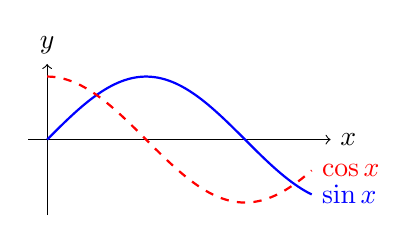
\begin{tikzpicture}[scale=0.8]
      \draw[->] (-0.3,0) -- (4.5,0) node[right] {$x$};
      \draw[->] (0,-1.2) -- (0,1.2) node[above] {$y$};
      \draw[domain=0:4.2, samples=80, blue, thick]
        plot (\x, {sin(\x r)}) node[right] {$\sin x$};
      \draw[domain=0:4.2, samples=80, red, thick, dashed]
        plot (\x, {cos(\x r)}) node[right] {$\cos x$};
    \end{tikzpicture}
  \end{center}
\end{frame}

\begin{frame}{表}
  \begin{table}
    \centering
    \begin{tabular}{lcc}
      \hline
      テーマ名    & カラー   & スタイル \\
      \hline
      Madrid      & seahorse & プロ向け \\
      Berlin      & beaver   & モダン \\
      Copenhagen  & whale    & シンプル \\
      \hline
    \end{tabular}
    \caption{代表的な Beamer テーマ}
  \end{table}
\end{frame}

% -------------------------------------------------------------------
% セクション 4: 2カラムレイアウト
% -------------------------------------------------------------------
\section{2カラムレイアウト}

\begin{frame}{2カラム}
  \begin{columns}
    \begin{column}{0.5\linewidth}
      \textbf{左カラム}
      \begin{itemize}
        \item 項目1
        \item 項目2
        \item 項目3
      \end{itemize}
    \end{column}
    \begin{column}{0.5\linewidth}
      \textbf{右カラム}
      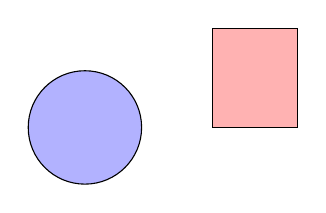
\begin{tikzpicture}[scale=0.9]
        \draw[fill=blue!30] (0,0) circle (0.8);
        \draw[fill=red!30]  (1.8,0) rectangle (3,1.4);
      \end{tikzpicture}
    \end{column}
  \end{columns}
\end{frame}

% -------------------------------------------------------------------
% 最終スライド
% -------------------------------------------------------------------
\begin{frame}{まとめ}
  \begin{block}{Beamer の主な機能}
    \begin{itemize}
      \item テーマ・カラーテーマで外観を変更
      \item \texttt{pause} / \texttt{onslide} で段階表示
      \item 数式・TikZ・表をそのまま利用
      \item \texttt{columns} で2カラムレイアウト
    \end{itemize}
  \end{block}

  \vspace{1em}
  \centering
  \Large ご清聴ありがとうございました
\end{frame}

\end{document}